%\subsection{Leptonically decaying boson}
\label{subsec:leptons_selection}

%%% 1-lepton channel
\label{subsubsec:1lep_event_selection}
%This section summarizes the SR definitions in 1-lepton channel.
%\textbf{$W \to \ell\nu$}

The event selections for this analysis are largely based on the methodology used in a previous study with the 36\,\ifb dataset~\cite{Ryzhov:2310214}.
In the \olep channel, events are required to contain a $\ell\nu$ pair indicative of a $W$ boson decay, along with a $W/Z \to q\bar{q}$ candidate. The candidate for the $W \to \ell\nu$ decay is identified by the presence of exactly one Tight lepton and the absence of any Loose leptons in the final state.

The following anti-QCD cuts are applied to reject the QCD multijet and non-collision background:
\begin{itemize}
\item $\met > 80 \,\GeV$
\item $\ptl > 28 \,\GeV$ 
\end{itemize}

%Merged and resolved regime selections are detailed in Section \ref{subsec:sr_selection}.
Figure \ref{fig:1LepPreselCuts} shows the distributions of missing transverse energy (\met), lepton transverse momentum (\ptl), and large-$R$ jet mass ($m_{J}$) in the 1-lepton channel at different stages of the analysis. The ``preselection merged'' and ``preselection resolved'' stages refer to the application of initial selection criteria in the merged and resolved regimes, respectively. These stages exclude the use of boson tagger cuts for the large-$R$ jet and mass window cuts for signal jets, which are detailed further in Section \ref{subsec:sr_selection}.

In the distributions before any event selection, the observed data that are not adequately represented by the simulated events primarily originate from multijet and non-collision backgrounds. These discrepancies mainly arise due to the mis-measurement of jet energy. Although these backgrounds are relatively minor, it is crucial to acknowledge that MC simulations do not accurately estimate their shape or rate. The multijet background, often referred to as the QCD background, typically occurs when jets are misidentified as leptons or when leptons are produced later in the decay process of jets.
Electron-related backgrounds are predominantly caused by jets generating extensive showers in the Electromagnetic Calorimeter (ECAL), which subsequently meet the criteria for electron trigger. For muons, the background typically arises from hadron decays within jets.
Therefore, events from either QCD multijet or non-collision backgrounds typically contain ``soft'' (low \( p_{T} \)) leptons, which are effectively suppressed by the reasonable requirements on \met and \ptl.
After the anti-QCD cuts, we observe good agreement between the data and MC simulation in both merged and resolved regimes. In the $m_{J}$ distribution, the $W$-peak in the $t\bar{t}$ process is also clearly visible.


\begin{figure}[ht]
\centering
        \begin{subfigure}{0.32\textwidth}
            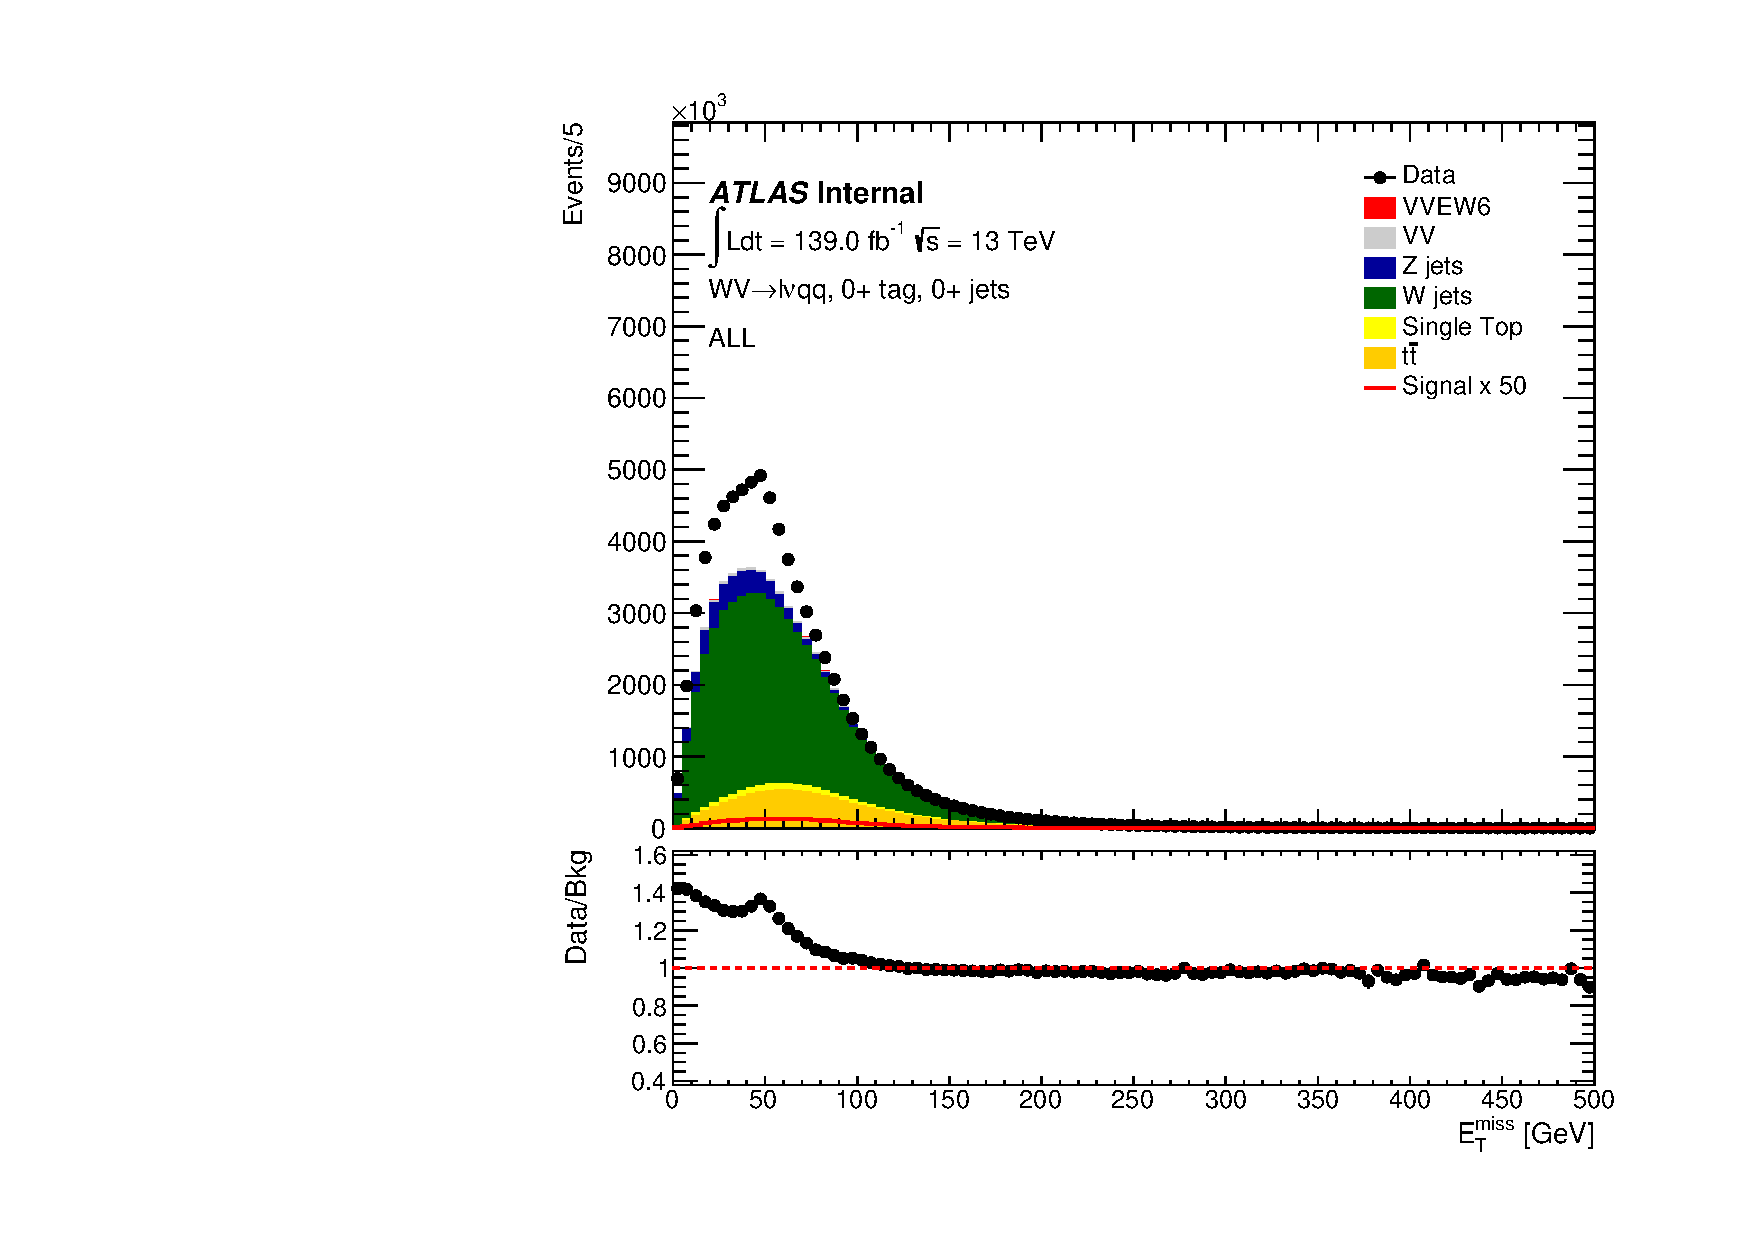
\includegraphics[width=\linewidth]{figures/event_selection/ALL_MET.pdf}
            \caption{$E_{T,miss}$ before any event selection.}
        \end{subfigure}
        \begin{subfigure}{0.32\textwidth}
            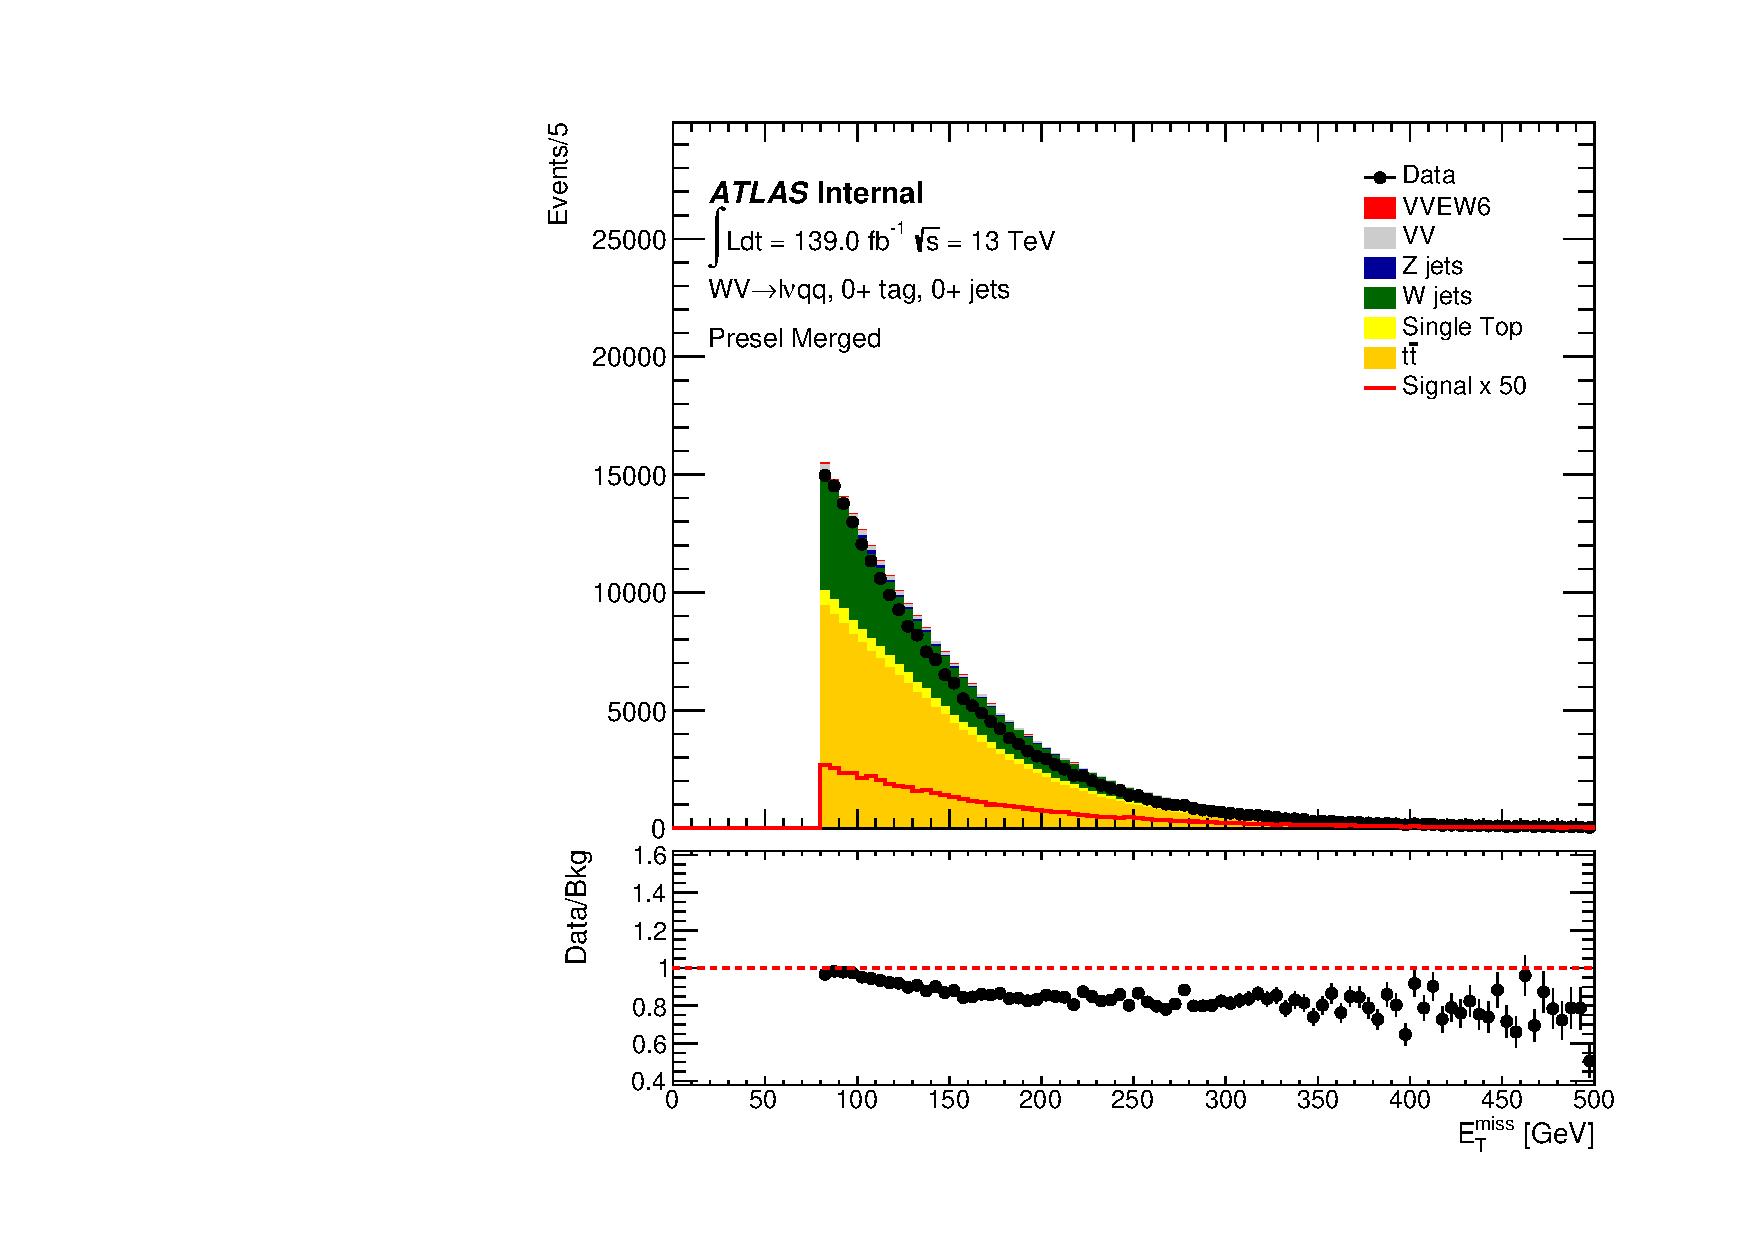
\includegraphics[width=\linewidth]{figures/event_selection/Presel_Merged_MET.pdf}
            \caption{$E_{T,miss}$ after merged common preselection.}
        \end{subfigure}
        \begin{subfigure}{0.32\textwidth}
            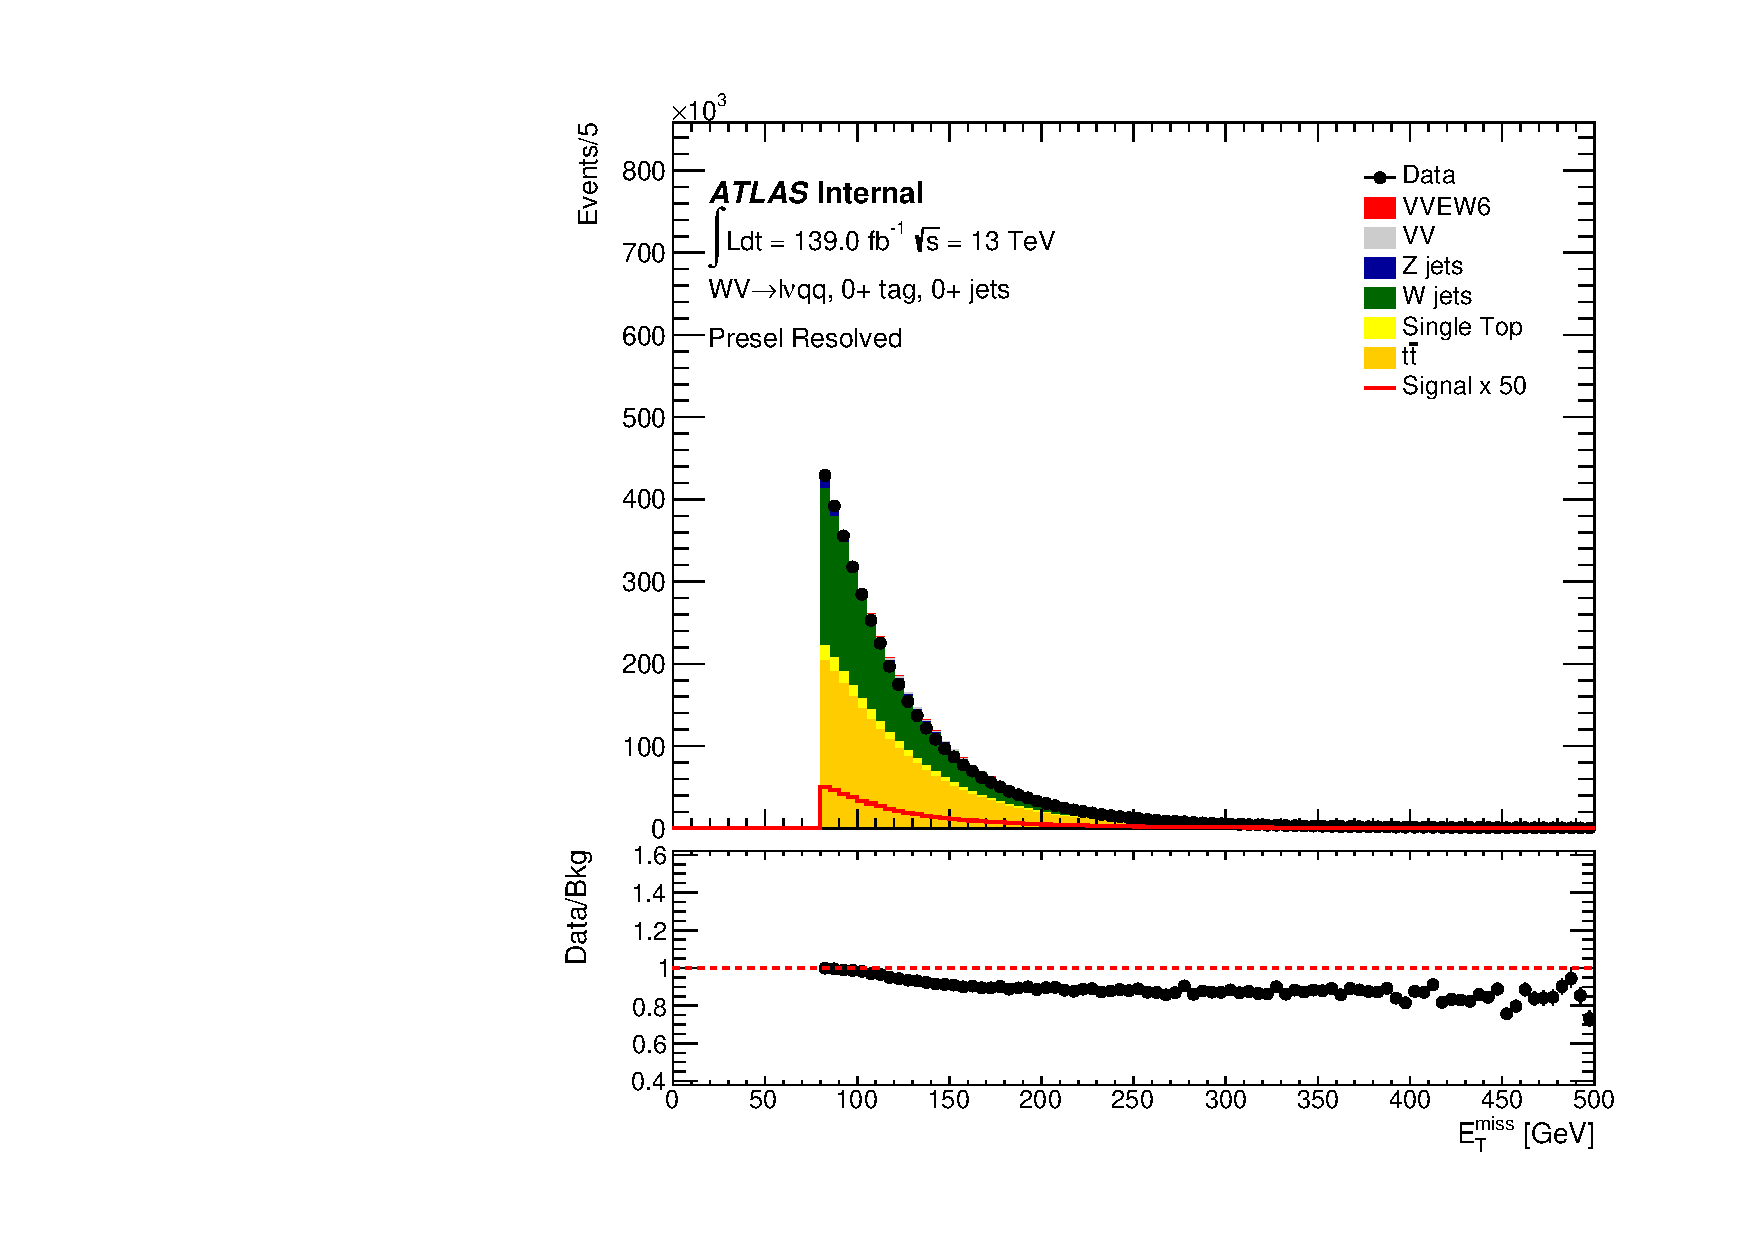
\includegraphics[width=\linewidth]{figures/event_selection/Presel_Resolved_MET.pdf}
            \caption{$E_{T,miss}$ after resolved common preselection.}
        \end{subfigure} \\

        \begin{subfigure}{0.32\textwidth}
            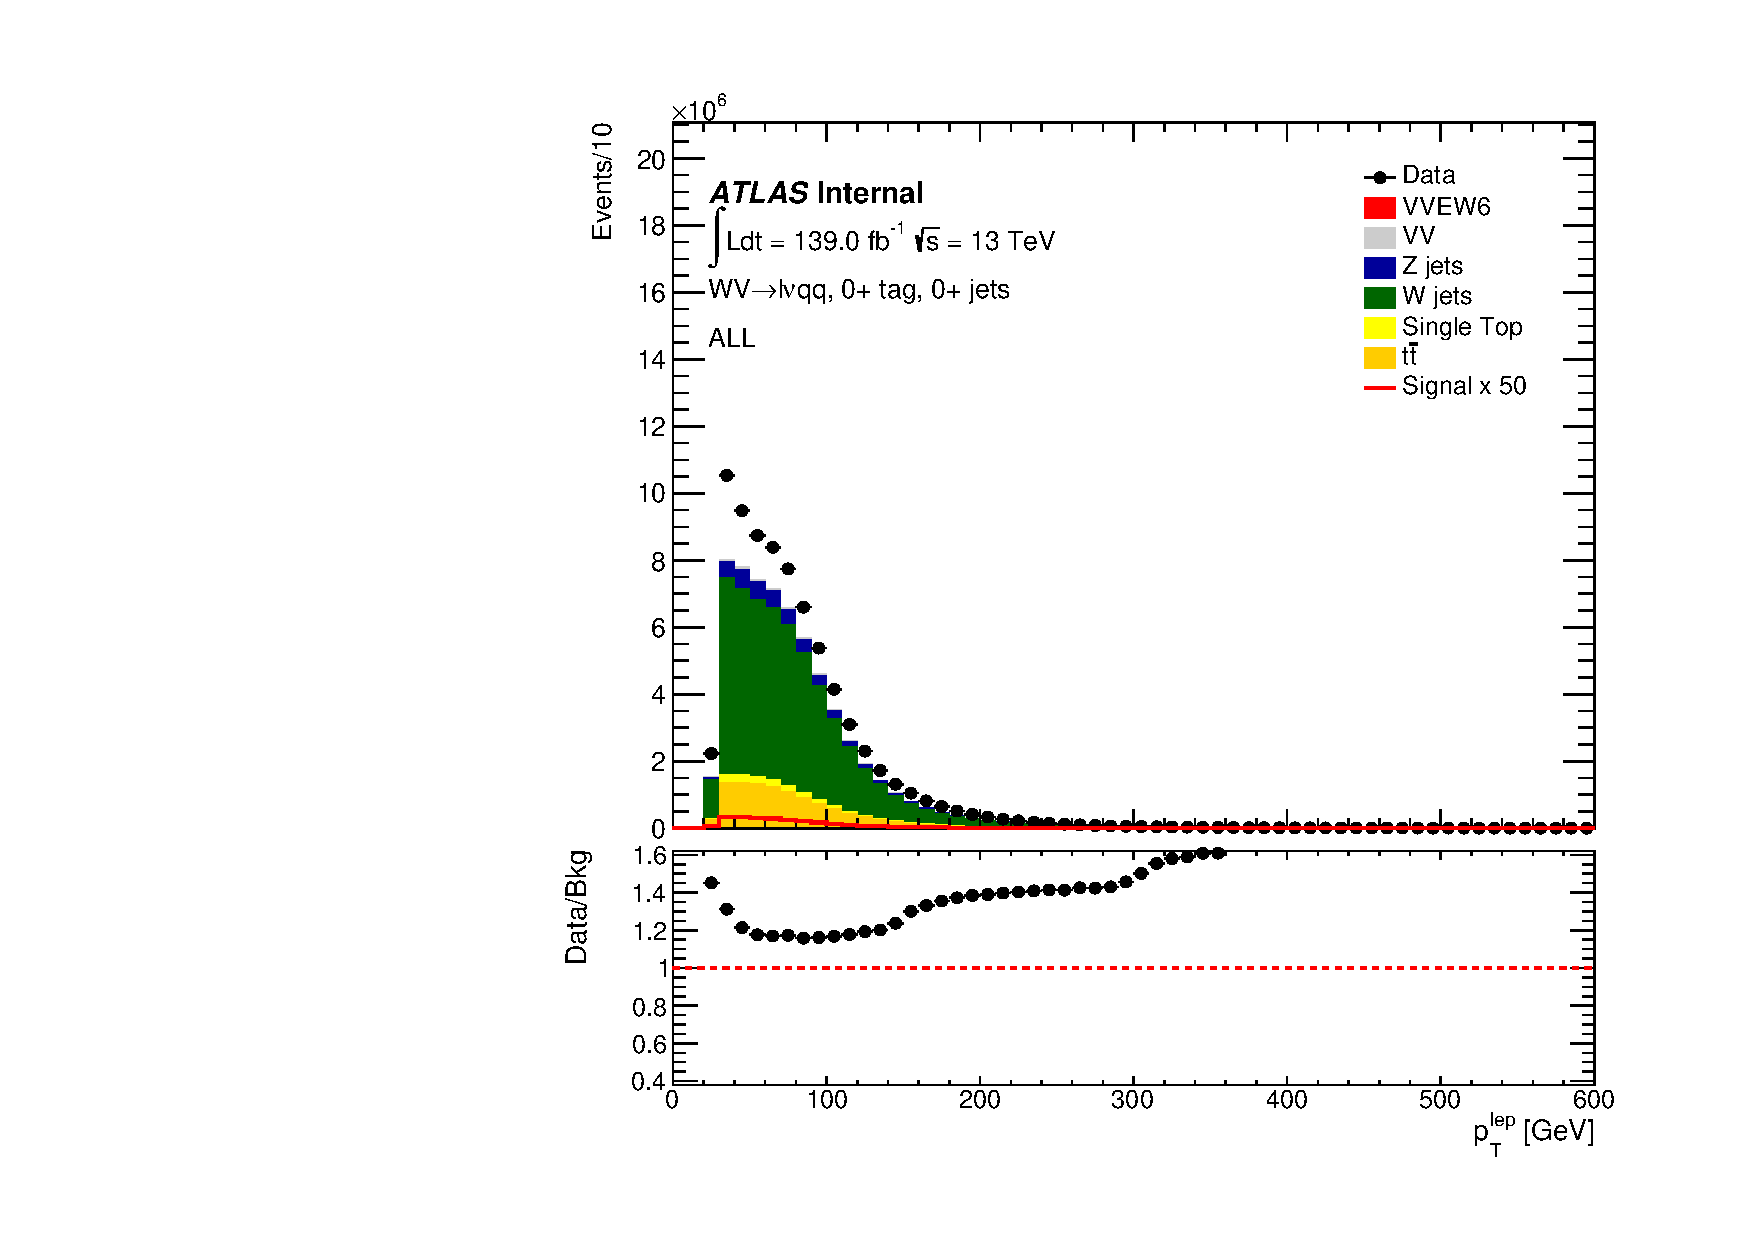
\includegraphics[width=\linewidth]{figures/event_selection/ALL_PtL.pdf}
	    \caption{$p_{T,l}$ before any event selection.\\ \hbox{\vspace{1.5mm}}}
        \end{subfigure}
        \begin{subfigure}{0.32\textwidth}
            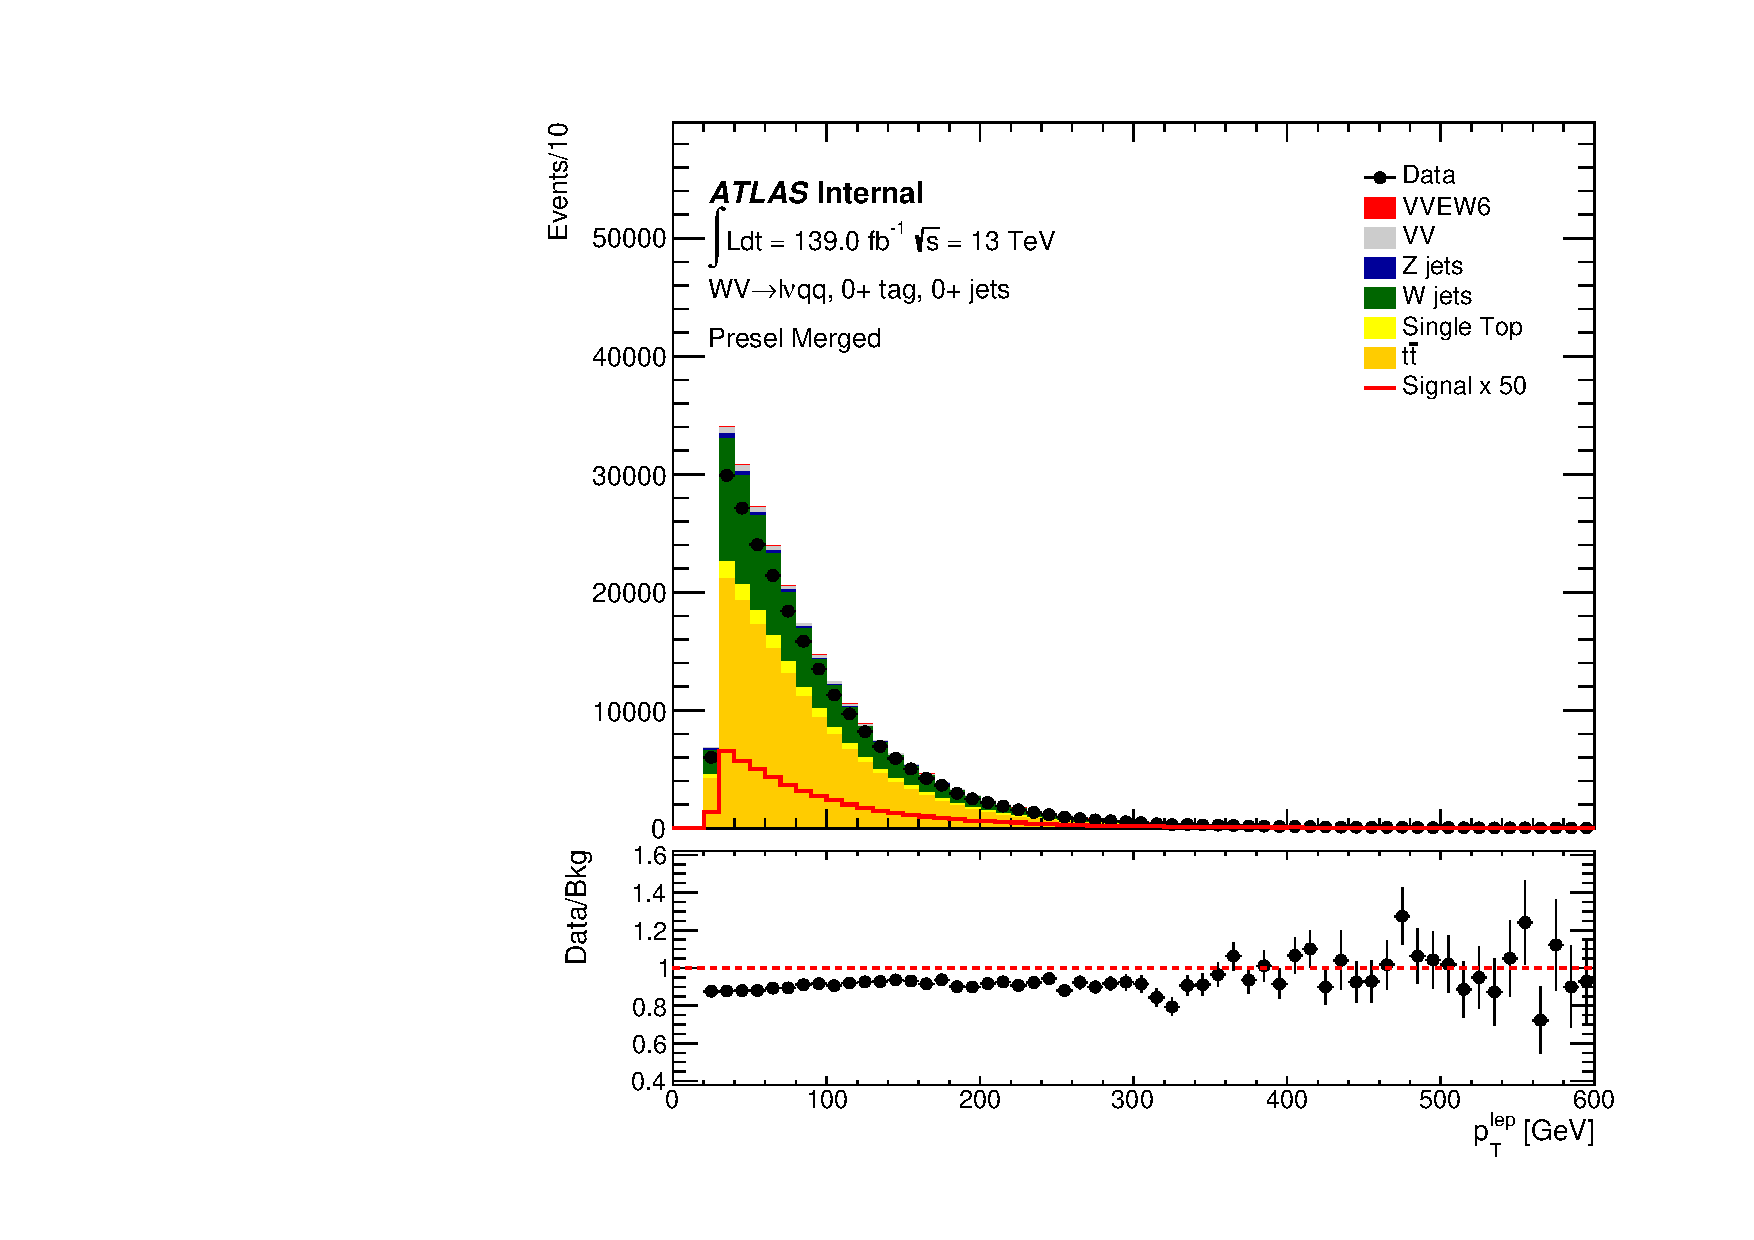
\includegraphics[width=\linewidth]{figures/event_selection/Presel_Merged_PtL.pdf}
            \caption{$p_{T,l}$ after merged common preselection.}
        \end{subfigure}
        \begin{subfigure}{0.32\textwidth}
            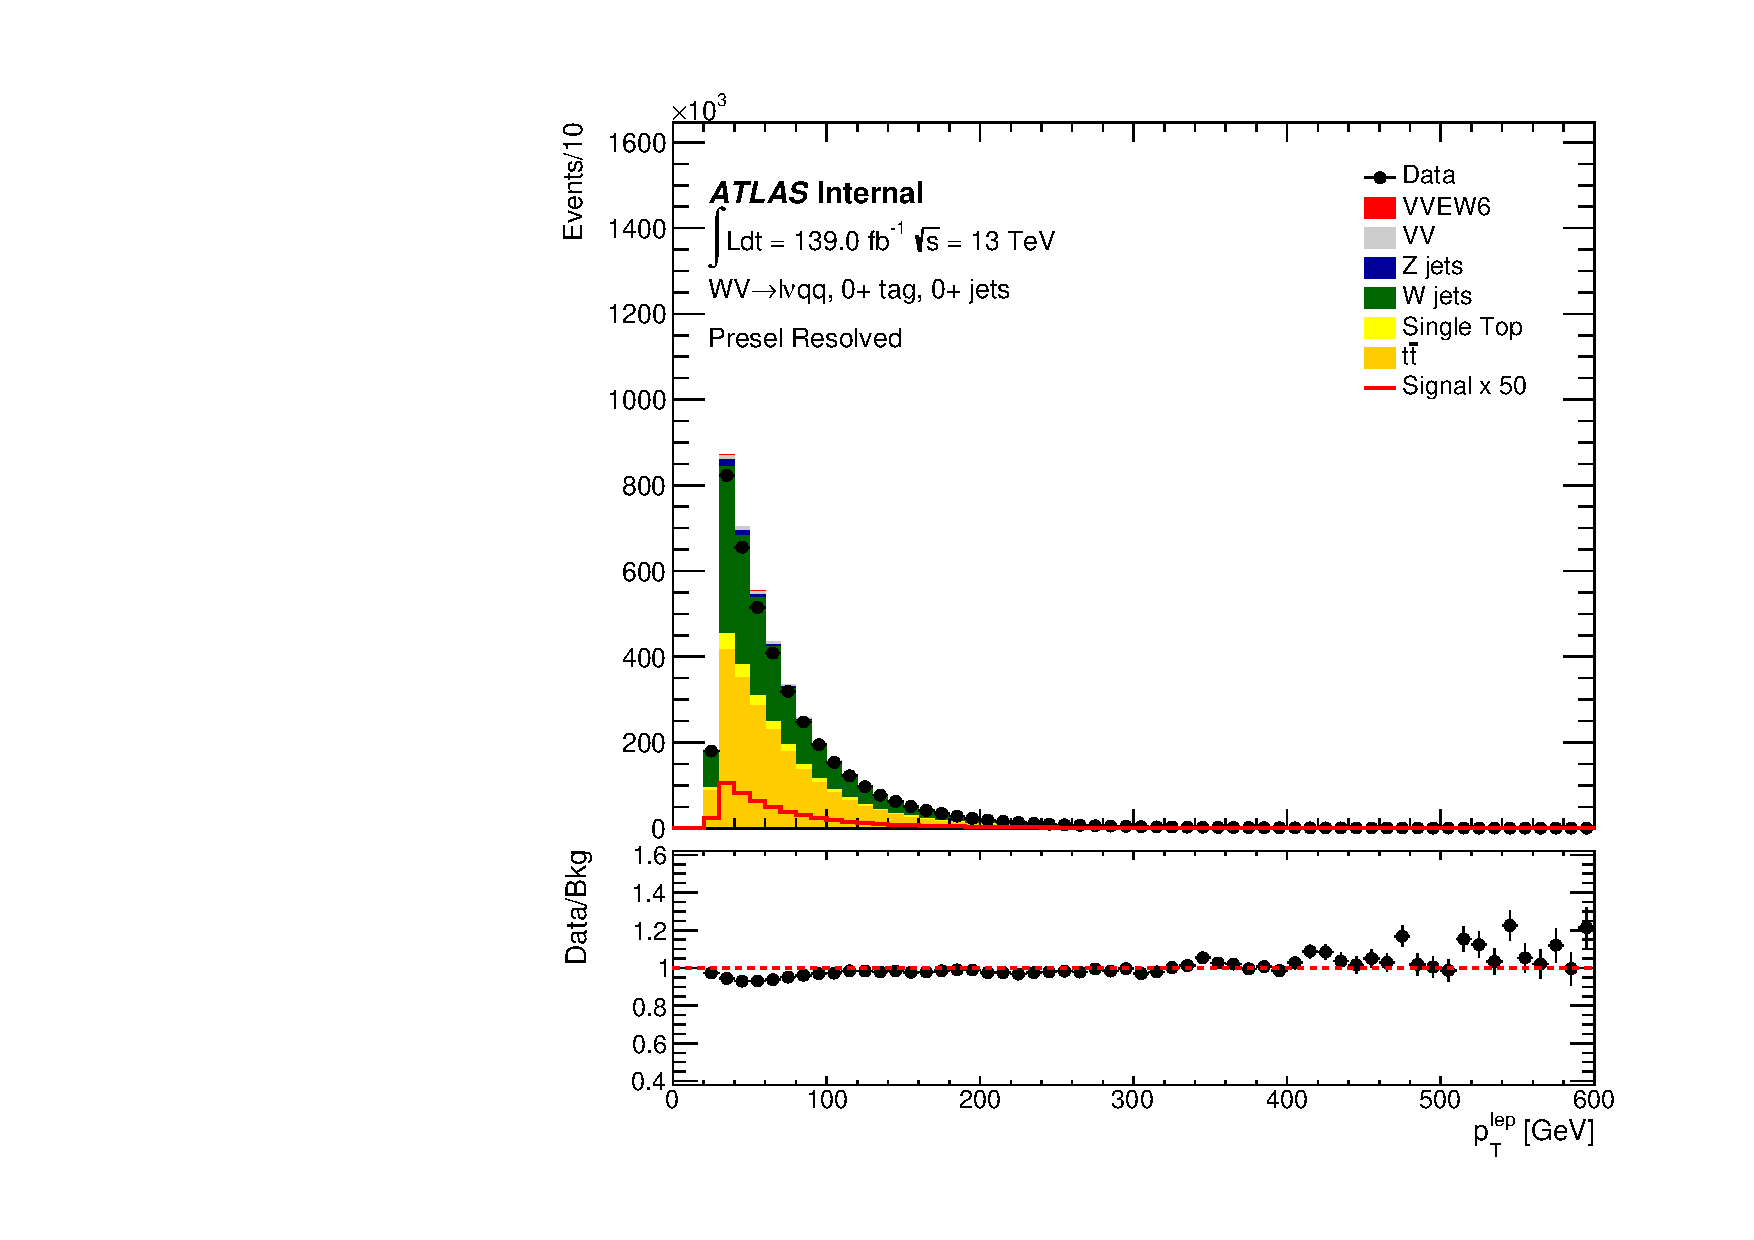
\includegraphics[width=\linewidth]{figures/event_selection/Presel_Resolved_PtL.pdf}
            \caption{$p_{T,l}$ after common resolved preselection.}
        \end{subfigure} \\

        \begin{subfigure}{0.32\textwidth}
            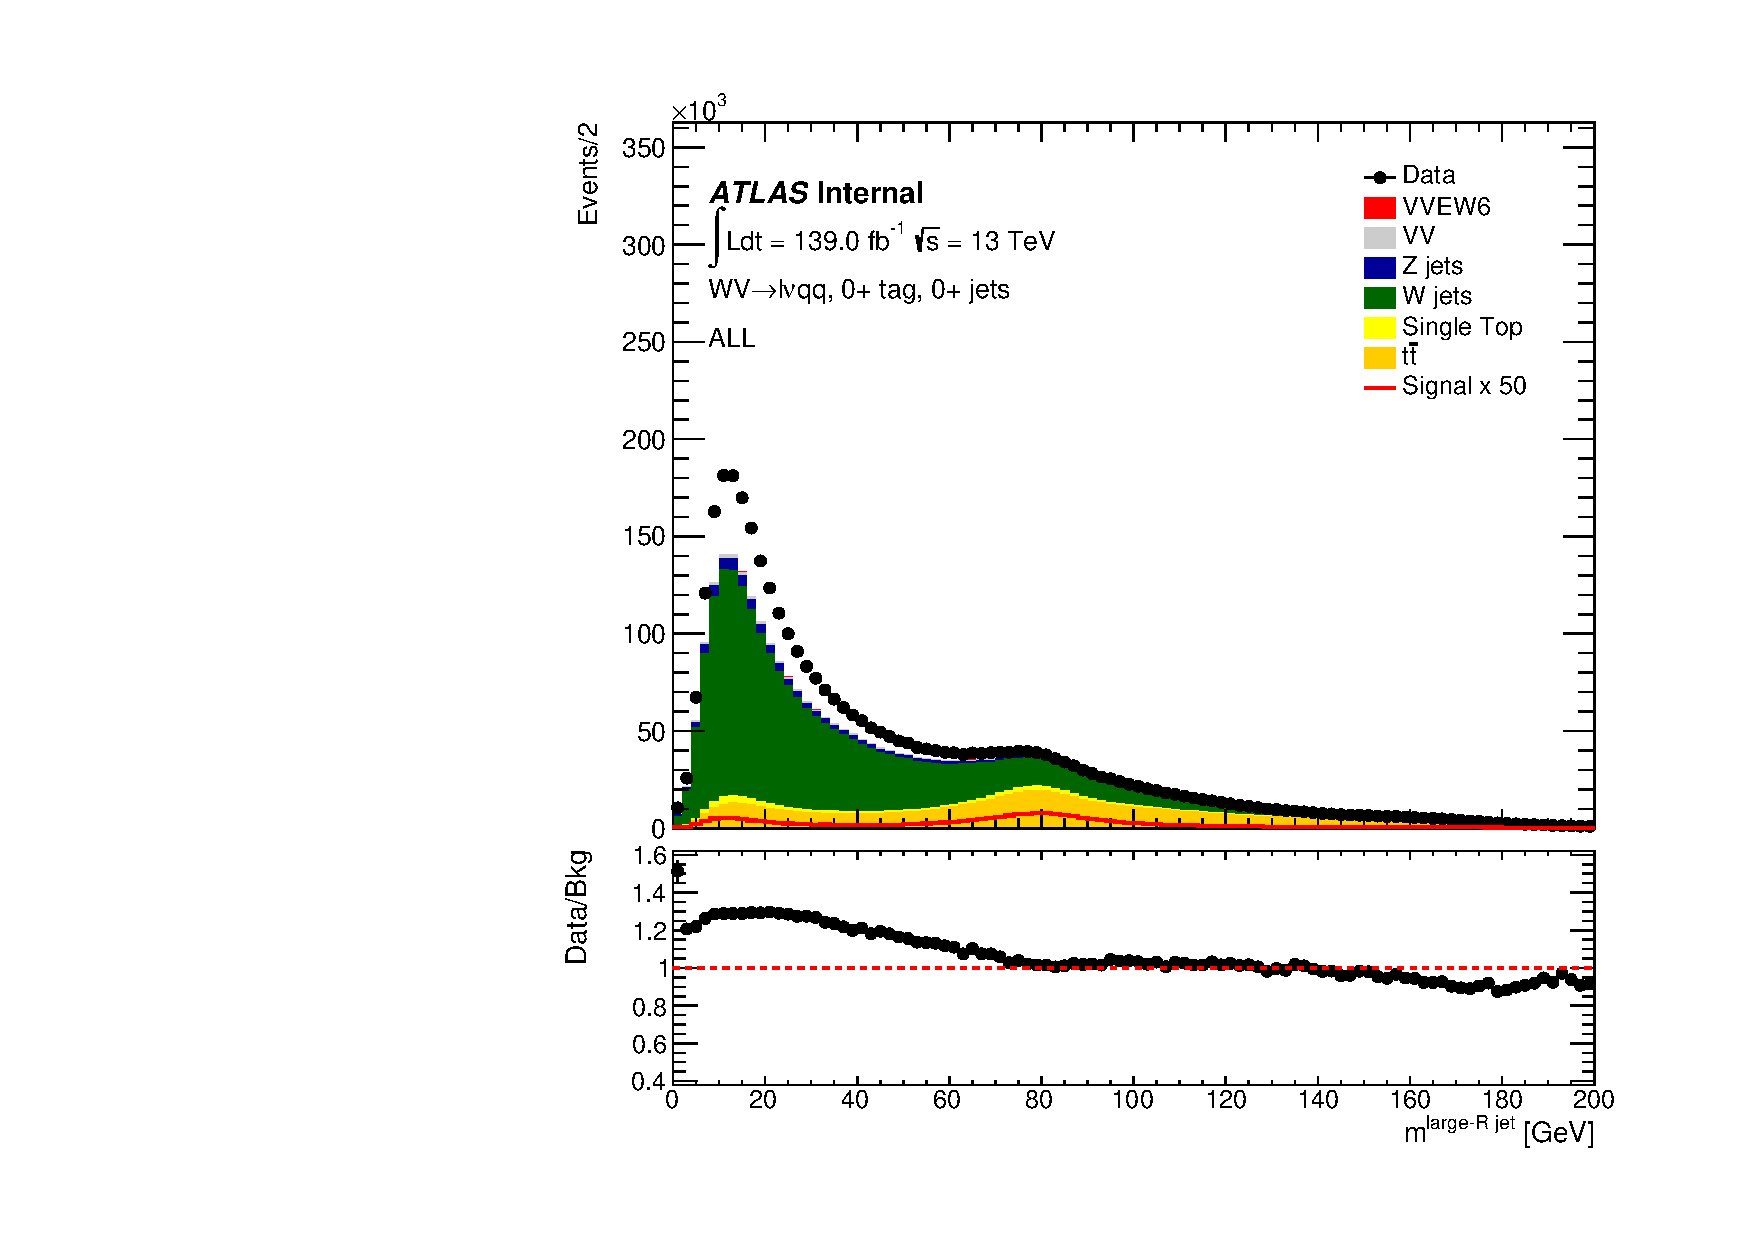
\includegraphics[width=\linewidth]{figures/event_selection/ALL_MFatJet.pdf}
	    \caption{$M_{J}$ before any event selection.\\ \hbox{\vspace{1.5mm}}}
        \end{subfigure}
        \begin{subfigure}{0.32\textwidth}
            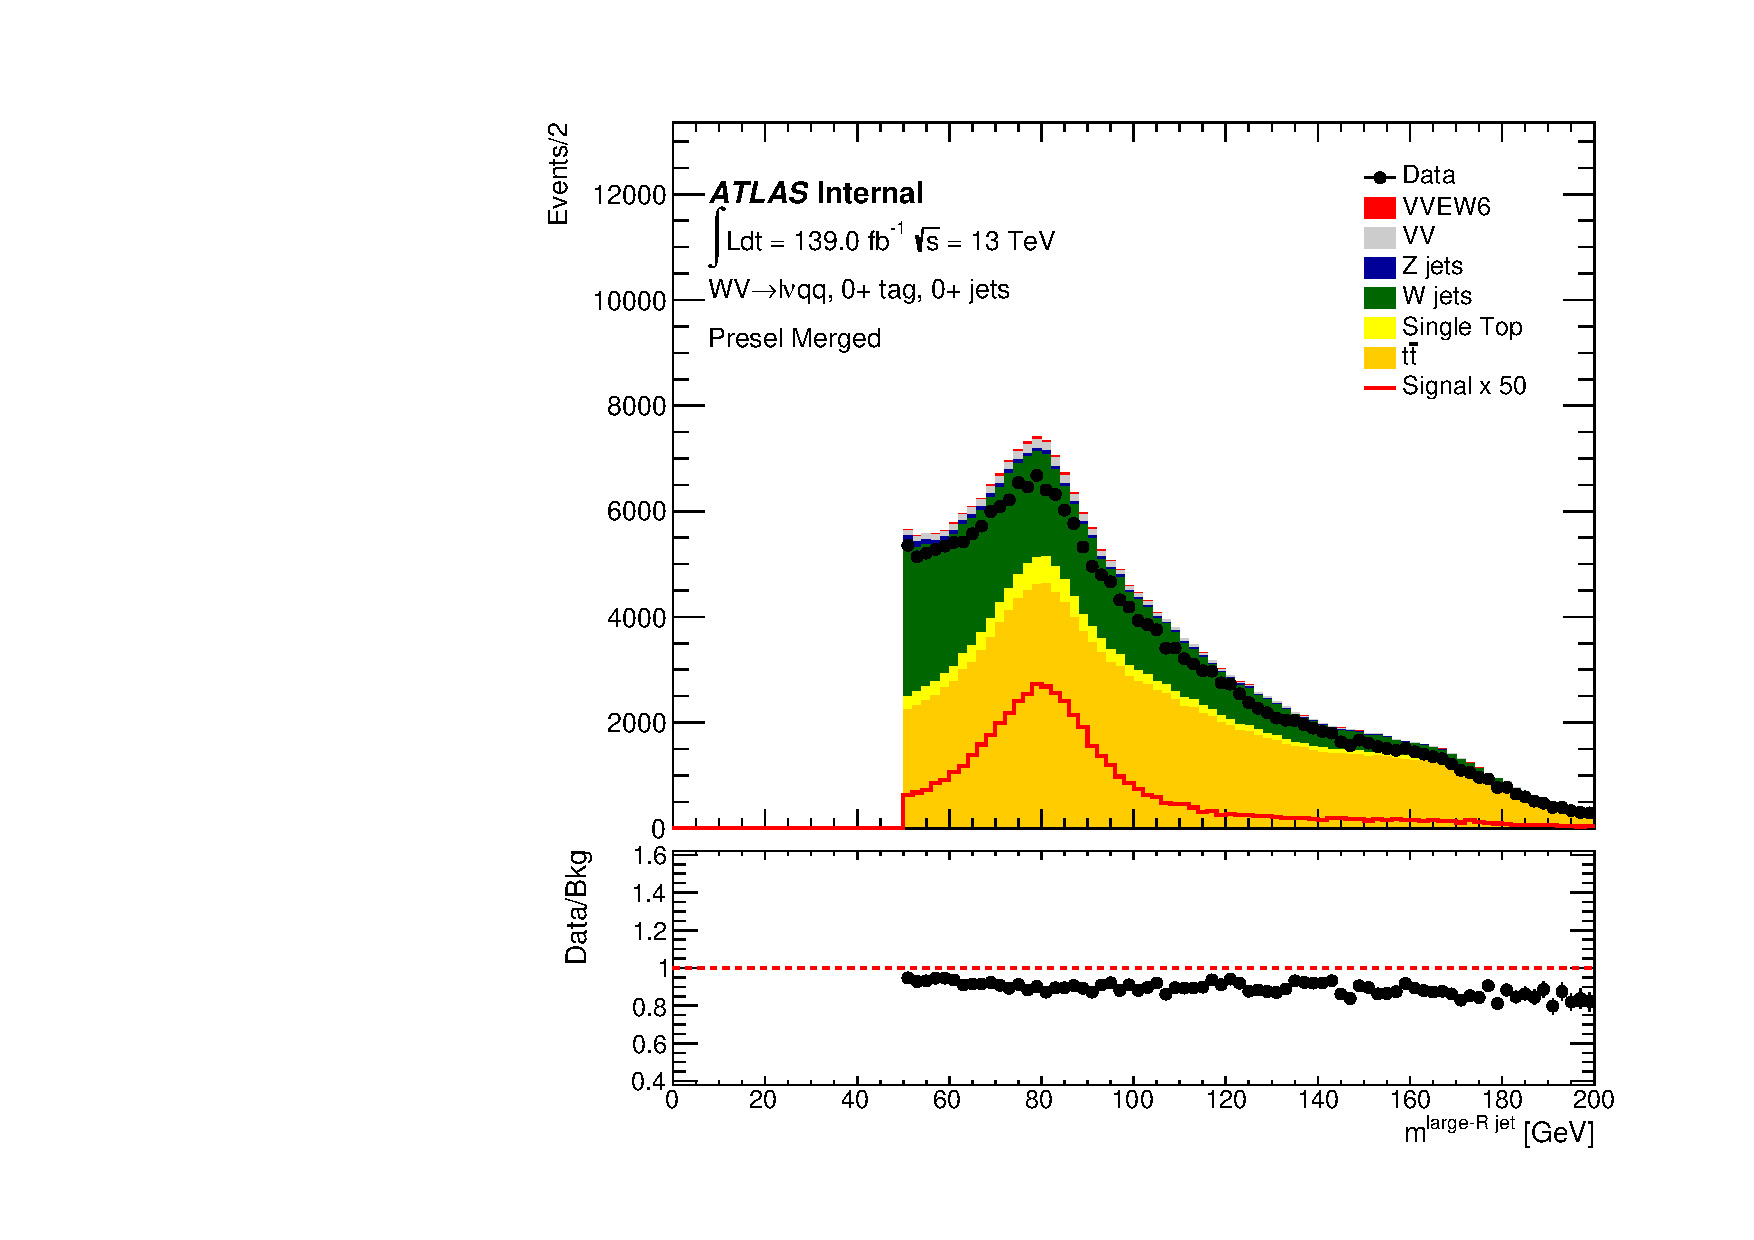
\includegraphics[width=\linewidth]{figures/event_selection/Presel_Merged_MFatJet.pdf}
            \caption{$M_{J}$ after merged common preselection.}
        \end{subfigure}
        \caption{Distributions of \met, \ptl, and $m_{J}$ in the 1-lepton channel at various analysis stages.}
	\label{fig:1LepPreselCuts}
\end{figure}
